\documentclass[a4paper,10pt]{report}

\usepackage[francais]{babel} %francais, polish, spanish, ...
\usepackage[T1]{fontenc}
\usepackage[utf8]{inputenc}
\usepackage{comment}
\usepackage[final]{pdfpages}
\usepackage{lmodern} %Type1-font for non-english texts and characters
\usepackage{graphicx} %%For loading graphic files
\usepackage{fancyhdr}

% Title Page
\title{Architecture}
\author{Jeremy Arrestier, Thibaut Fabre, Alexandre Kervadec, Guillaume Verdugo}


\begin{document}
\maketitle

  \begin{figure}[ht]
  \begin{center}
   \fbox{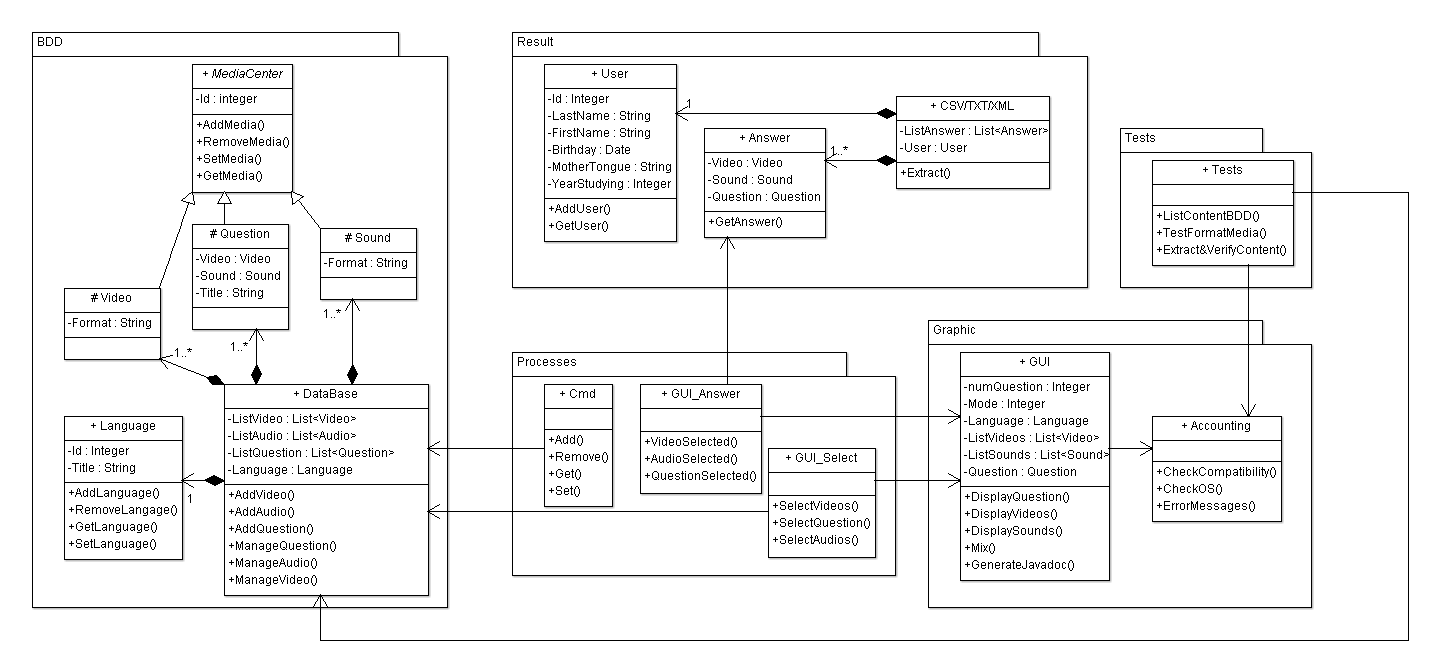
\includegraphics[width=18cm,angle=90]{architecture.png}}
   \caption{UML - Architecture}
   \label{diaglog} 
  \end{center}
  \end{figure}
  
  \section{Explication détaillée de l'UML}
  
  Notre architecture est structuré en plusieurs grands groupes se composant de classes. Nous allons décrire ces groupes un à un.
  
  \subsection{BDD}
  
  Ce package contient l'ensemble des médias qui seront disponibles sur l'application (audio, vidéos, questions, langue de la question).
  
  Cette organisation des données a été choisie pour optimiser l'ajout de médias et pour permettre l'ajout d'autres langues à l'application.
  
  \subsection{Result}
  
  Ce package-ci est l'ensemble des informations concernant l'utilisateur (le sujet de l'expérience). Il est aussi composé de ses résultats aux réponses du test ainsi que d'une classe permettant d'extraire les données vers un fichier \textit{CSV / txt / XML}.
  
  \subsection{Tests}
  
  Ce package regroupe l'ensemble des tests qui seront necessaires pour minimiser les erreurs au niveau de la base de données (par exemple lors d'un upload de médias, on vérifie que le format soit adapté).
  
  \subsection{Graphic}
  
  Ici sont regroupés toutes les fonctionnalités liées à l'interface graphique.
  
  \subsection{Processes}
  
  Nous avons réuni ici, tout ce qui correspond au \textit{contrôleur} de l'application.
  
  La classe \textbf{GUI\_select} est la sélection de l'ensemble des médias présentées lors d'une question.
  \textbf{GUI\_Answer} correspond à la vidéo et à l'audio sélectionnés par l'utilisateur liés à une question.
  
  \textbf{Cmd} est l'utilisation de l'application par l'administrateur lorsqu'il voudra ajouter ou retirer des médias et questions de la base de données.
  
 

  
\end{document}          
